\section{三角函数}\label{005}

\begin{flushright}{\kaishu 道可道, 非常道; 名可名, 非常名.}\end{flushright}

\begin{tcolorbox}[size=fbox, breakable, enhanced jigsaw, title={三角函数
(trigonometry)}]

三角函数最基本的使用应该是表示直角三角形的变长比. 如下图所示, 三角形
$ABC$ 为直角三角形, 将 $\angle BAC$ 记作 $\theta$, 对于两条直角边
$AB$ 和 $BC$, 边 $AB$ 在 $\theta$ 边上, 称它为\textbf{邻边}
(adjacent), 边 $BC$ 在 $\theta$ 对面, 称它为\textbf{对边}
(opposite), 剩余的边 $AC$ 被称为\textbf{斜边} (hypotenuse)。

\begin{tcolorbox}[size=fbox, breakable, enhanced jigsaw]
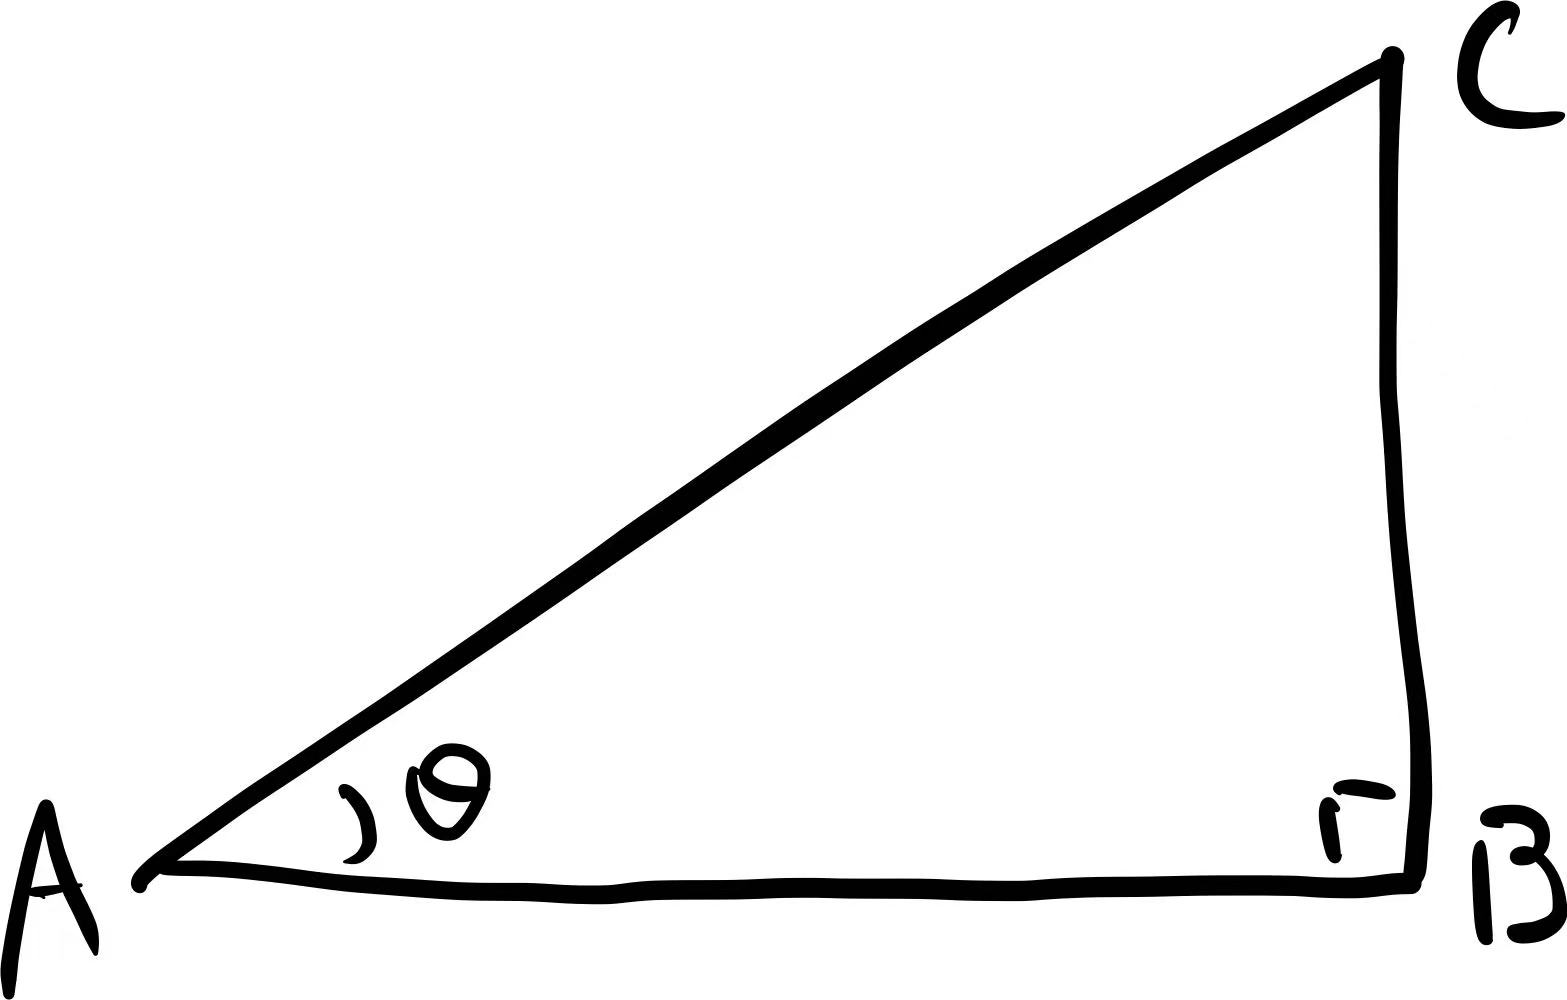
\includegraphics[width=0.5\textwidth]{img/image-20230308142717670.png}
\end{tcolorbox}

易见, 各变长比仅和 $\theta$ 相关\footnote{当然也可以说和除了直角外的另一个角
  $(90^\circ-\theta)$ 相关; 边长比可以通过一个除直角外的角确定是因为,
  除直角外另一角相等的直角三角形都相似, 它们的边长比是一致的。},
三角函数便是用来表示各个比例的, 常用的三角函数有

$\begin{aligned}\cos\theta&=\frac{\text{邻边}}{\text{斜边}}=\frac{AB}{AC},\\ \sin\theta&=\frac{\text{对边}}{\text{斜边}}=\frac{BC}{AC},\\ \tan\theta&=\frac{\text{对边}}{\text{邻边}}=\frac{BC}{AB}.\end{aligned}$

不难看出$\tan\theta=\frac{\sin\theta}{\cos\theta}$.

另外还有

$\begin{aligned}\sec\theta&\equiv\frac{1}{\sin\theta},\\ \csc\theta&\equiv\frac{1}{\cos\theta},\\ \cot\theta&\equiv\frac{1}{\tan\theta}.\end{aligned}$

$\csc$ 很多时候也记作 $\text{cosec}$.

一个非常实用的关系, 直角三角形中有\textbf{勾股定理} (Pythagorean
theorem): 斜边边长平方等于两直角边边长的平方之和, 即 $AC^2=AB^2+BC^2$;
两边同时除以 $AC^2$ 便有

\begin{itemize}

\item
  $\boxed{1=\cos^2\theta+\sin^2\theta}$.\footnote{三角函数的平方:
    cos(x)\textsuperscript{2} 通常理解为 cos((x)\textsuperscript{2});
    cos\textsuperscript{2}x 约定俗成表示 (cos(x))\textsuperscript{2}.}
\end{itemize}

\end{tcolorbox}

\begin{tcolorbox}[size=fbox, breakable, enhanced jigsaw, title={反三角函数}]

三角函数, 输入一个角度, 返回一个边长比; 反三角函数便是三角函数得逆运算,
或者说反函数 (参见\ref{004}\nameref{004}), 即输入一个边长比, 返回一个角度.

\end{tcolorbox}

\begin{tcolorbox}[size=fbox, breakable, enhanced jigsaw, title={正弦定律 (law of sine)}]

将三角形三个角分别记作 $\alpha$, $\beta$, 和 $\gamma$,
将它们的对边分别记作 $A$, $B$, 和 $C$. 先是结论:

\begin{itemize}

\item
  $\boxed{\frac{A}{\sin\alpha}=\frac{B}{\sin\beta}=\frac{C}{\sin\gamma}}$.
\end{itemize}

\begin{tcolorbox}[size=fbox, breakable, enhanced jigsaw]
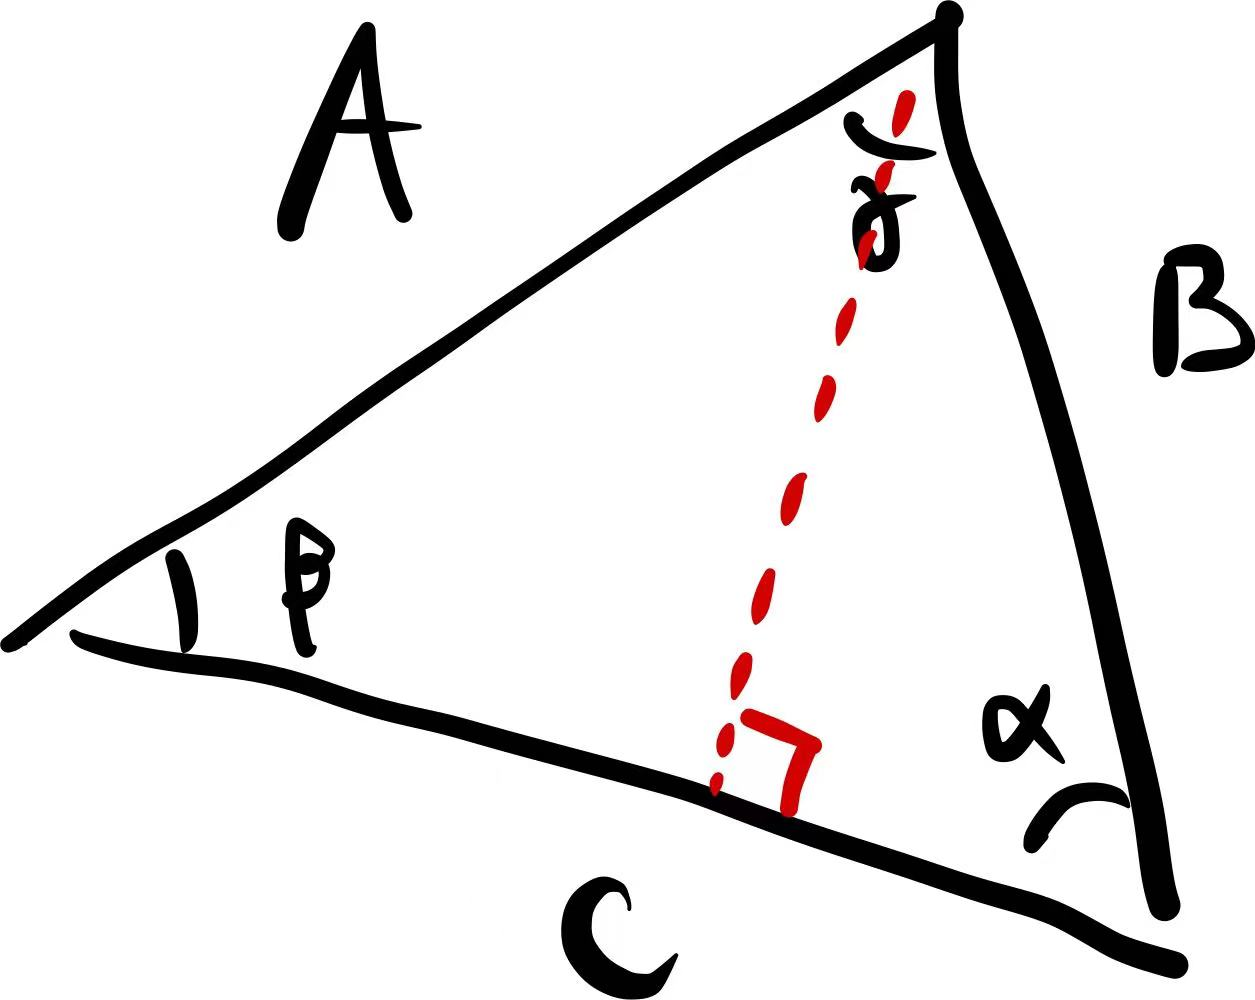
\includegraphics[width=0.5\textwidth]{img/image-20230308142913522.png}
\end{tcolorbox}

推导如下:

如上图所示, 以 $C$ 为底做高, 将原本的三角形分为左右两个直角三角形,
这条高利用左边的直角三角形可以表示为 $A\sin\beta$,
利用右边的直角三角形则是 $B\sin\alpha$, 于是有
$A\sin\beta=B\sin\alpha$, 整理可得
$\frac{A}{\sin\alpha}=\frac{B}{\sin\beta}$;
再做另一条高重复前面的操作, 便可得到完整的结论.

\end{tcolorbox}

\begin{tcolorbox}[size=fbox, breakable, enhanced jigsaw, title={余弦定律 (law of cosine)}]

还是先上结论:

\begin{itemize}

\item
  $\boxed{B^2=A^2+C^2-2AC\cos\beta}$,
\end{itemize}

即, 【一条边的边长平方】等于【另两条边的边长平方之】和加上【两倍的
(另两条边边长的乘积) 乘以 (另两条边的夹角的余弦)】.

\begin{tcolorbox}[size=fbox, breakable, enhanced jigsaw]
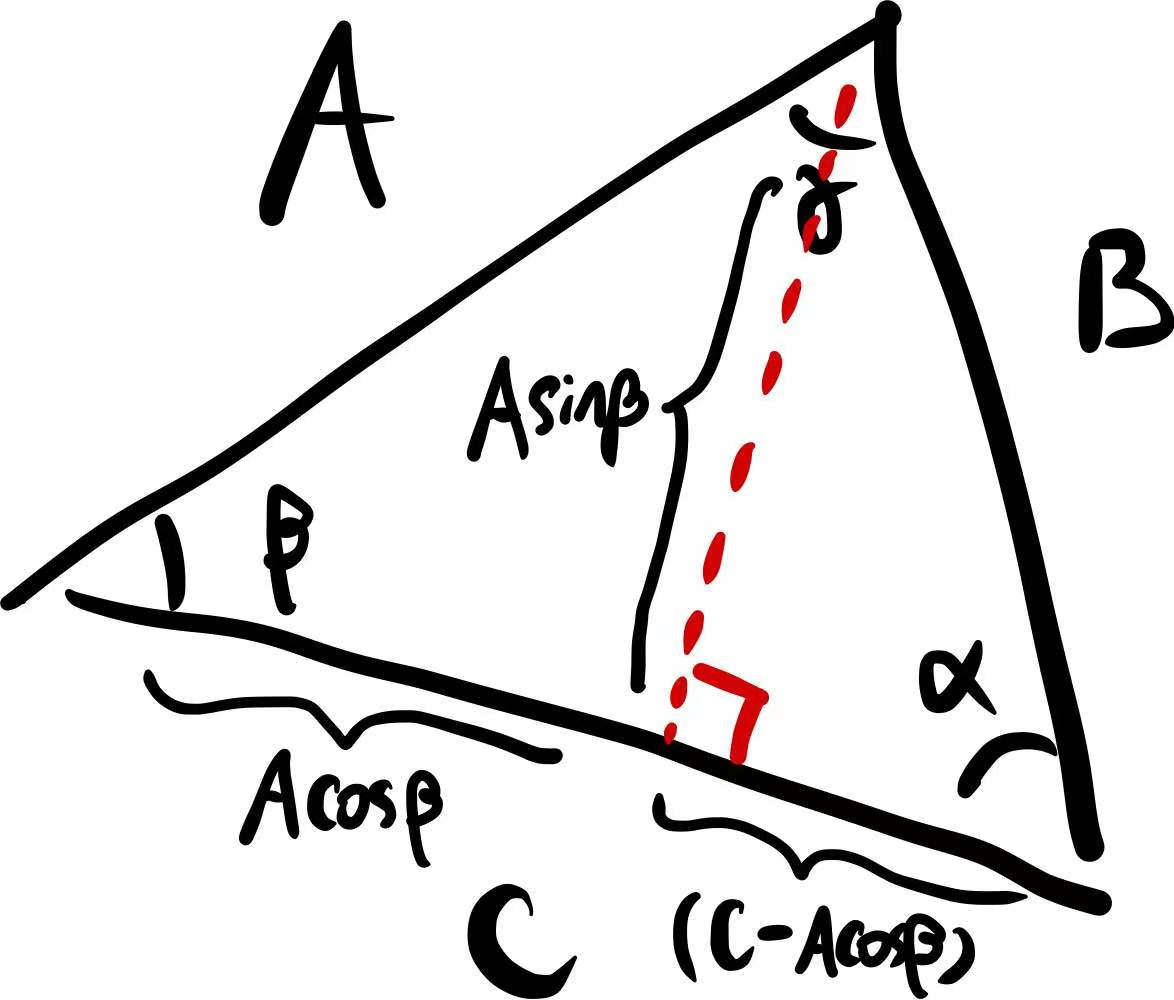
\includegraphics[width=0.5\textwidth]{img/image-20230308151417631.png}
\end{tcolorbox}

推导如下:

如下图所示, 依旧利用底边 $C$ 上的高将其分为左右两个直角三角形;
左边的直角三角形, 利用斜边 $A$ 和角 $\beta$, 两直角边分别可以表示为
$A\cos\beta$ 和 $A\sin\beta$, 于是右边的直角三角形边长便可表述为
$A\sin\beta$ 和 $(C-A\cos\beta)$; 对右边的直角三角形使用勾股定理

$\begin{aligned}B^2&=A^2\sin^2\beta+(C-A\cos\beta)^2\\ &=A^2\sin^2\beta+C^2+A^2\cos^2\beta-2AC\cos\beta\\ &=A^2+C^2-2AC\cos\beta.\end{aligned}$

其中等式的后两行用到了之前得出的 $1=\cos^2\theta+\sin^2\theta$.

\end{tcolorbox}

\begin{tcolorbox}[size=fbox, breakable, enhanced jigsaw, title={任意角度的三角函数}]

不难发现, 前面讨论的情况似乎都是锐角的情况 (主要是因为插图\ldots),
钝角的三角函数似乎没那么直观了, 因为做不成一个含有钝角的直角三角形,
没法简单地用边长比来表示 $\sin$ 和 $\cos$ 等. 于是,
我们需要想办法将前面的情形推广.

如下左图所示, 建立直角坐标系, 做一圆心位于原点的单位圆, 即半径为 $1$
的圆, 考虑在第一象限的圆上的一点, 将其与原点做连线, 将从
$x$-轴正方向与这条连线\textbf{顺时针}方向形成的夹角记作 $\theta$,
不难看出这个点的坐标 $(x,y)$ 满足

$\begin{cases}x=\cos\theta,\\y=\sin\theta.\end{cases}$

\begin{tcolorbox}[size=fbox, breakable, enhanced jigsaw]
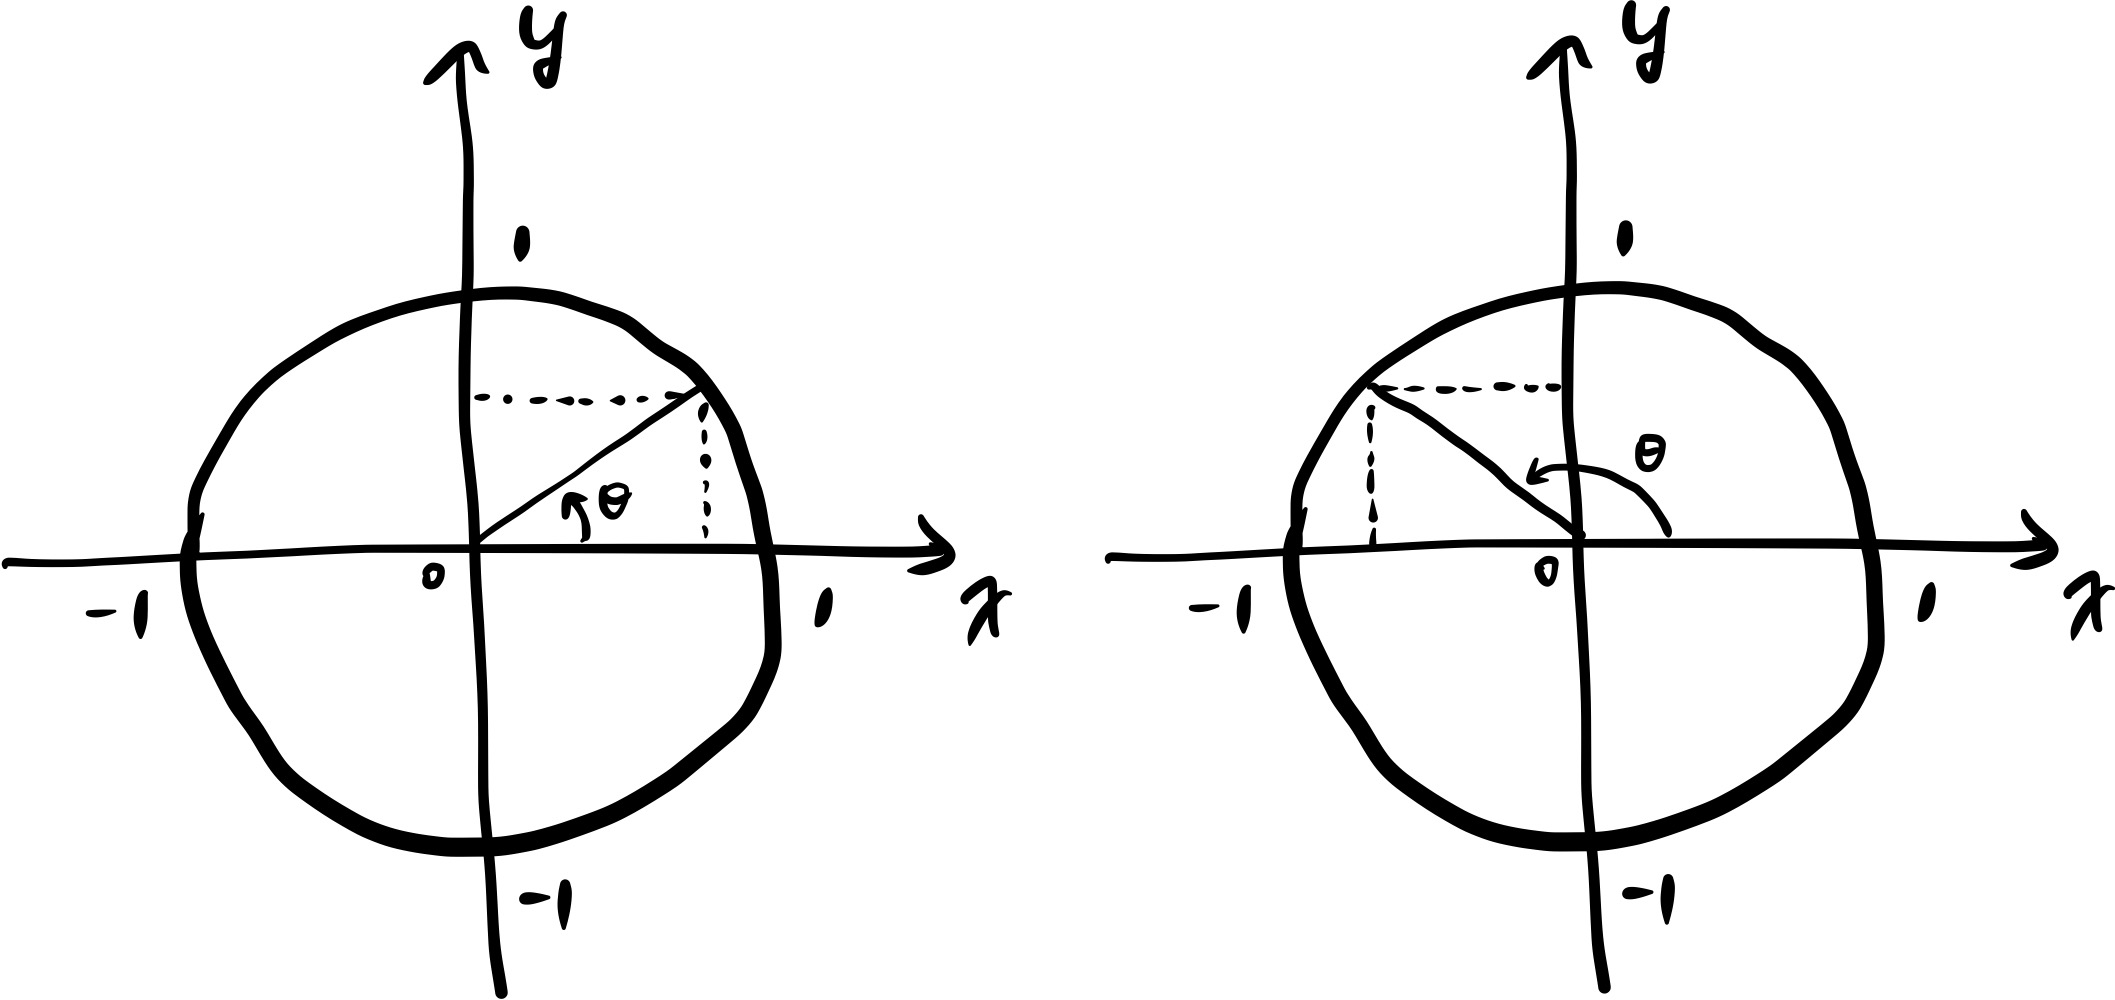
\includegraphics[width=0.75\textwidth]{img/image-20230316171124433.png}
\end{tcolorbox}

于是不妨将其他象限的情况也按此定义,
于是如上右图所示的钝角甚至更大角度的三角函数便可以被定义了.

\end{tcolorbox}

\begin{tcolorbox}[size=fbox, breakable, enhanced jigsaw, title={弧度制 (radian)}]

为什么一个周角是 $360^\circ$ 呢, 听说过一个不可考的说法: $360$
是一个有很多因数的数字 (1, 2, 3, 4, 5, 6, 8, 9, 10, 12\ldots),
等分起来的时候数字会比较友好, 所以 $360^\circ$ 其实是非常随意地规定的.
那么有没有更好的用来描述角度方法呢? 答案是弧度.

一个半径为 $r$ 的圆的周长是 $2\pi r$, 一个圆心角为 $n^\circ$
的扇形的弧长是 $2\pi r\frac{n}{360}$. 可见圆心角越大弧越长,
且圆心角和弧长成正比. 既然如此,
不如重新将角度定义为圆心角与弧长的比值以方便计算, 于是便有了,
在新的这套单位系统中, 若圆心角大小为 $\theta$, 其对应弧长应为
$r\theta$; 当圆心角是一个周角时, 对应弧长便成了圆的周长 $r(2\pi)$.
所以角度和这个新的单位的换算有 $360^\circ\equiv 2\pi\ \text{rad}$,
因为这个单位把圆心角和对应的弧长联系起来了, 因此称之为\textbf{弧度}
(radian).

扇形面积在这套单位制, 即弧度制下, 便也成了 $\frac{1}{2}r^2\theta$.

\end{tcolorbox}

\begin{tcolorbox}[size=fbox, breakable, enhanced jigsaw, title={三角函数的图像}]

现在这个时代, 大家都或多或少能接触到科学计算器,
再不济在bing.com上搜索``solver''用微软的 Microsoft Solver
也可以计算某个特定角度的三角函数值, 自然也可以绘制函数图像.
下图分别展示了 $\sin(x)$ 和 $\cos(x)$ 的图像,

\begin{tcolorbox}[size=fbox, breakable, enhanced jigsaw]
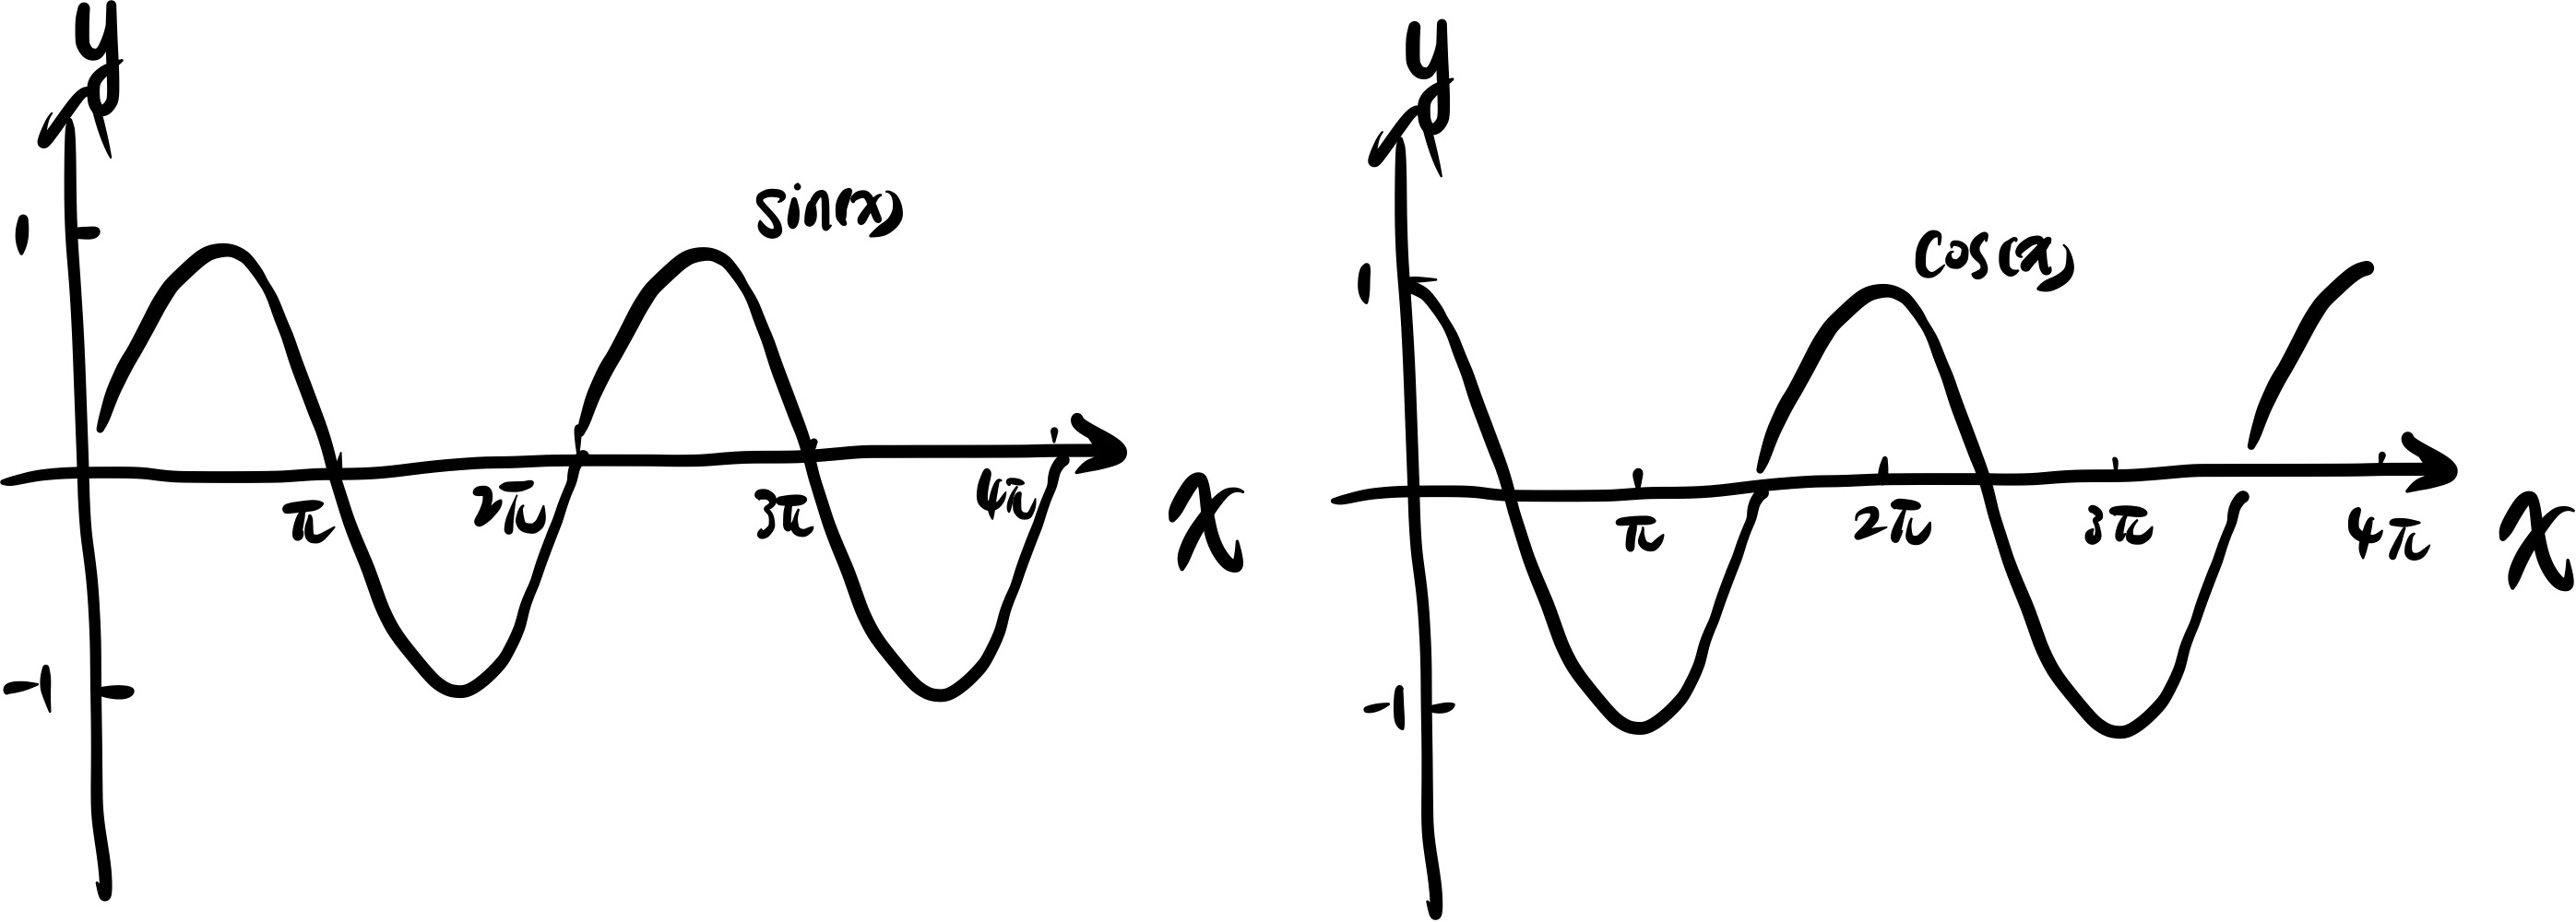
\includegraphics[width=0.75\textwidth]{img/image-20230316171137500.png}
\end{tcolorbox}

一些值得关注的点是它们都是\textbf{周期函数} (periodic function),
随着自变量-角度的变化, 因变量-函数值的变化是周期性的, 它们的周期都是
$2\pi$, 这一点从上文的单位圆里便可看出些许原因,
当角度变化超过一个周角时, 和角度刚从 $0$ 开始的情况是一样的.

\end{tcolorbox}